\documentclass[tikz,border=8pt]{standalone}
% Shared look for every TikZ diagram. Load with \input{../../tools/tikz-style.tex}
\usepackage[T1]{fontenc}
\usepackage{lmodern}
\renewcommand{\sfdefault}{lmr}  % diagrams use the same serif as the text
\usetikzlibrary{arrows.meta, positioning, shapes.geometric, calc, fit, backgrounds}
\definecolor{cblue}{HTML}{4C78A8}
\definecolor{corange}{HTML}{F58518}
\definecolor{cgreen}{HTML}{54A24B}
\definecolor{cred}{HTML}{E45756}
\definecolor{cpurple}{HTML}{B279A2}
\definecolor{cgrey}{HTML}{6B6B6B}
\tikzset{
  every picture/.style={font=\sffamily, line width=1.2pt},
  box/.style={draw=#1, fill=#1!12, rounded corners=4pt, align=center, inner sep=7pt, minimum height=1.1cm},
  box/.default=cgrey,
  arrow/.style={-{Stealth[length=3mm]}, draw=cgrey, line width=1.4pt},
  title/.style={font=\sffamily\bfseries\Large},
  note/.style={font=\sffamily\small, text=cgrey, align=center},
}
\AtBeginDocument{\hyphenpenalty=10000 \exhyphenpenalty=10000}

\begin{document}
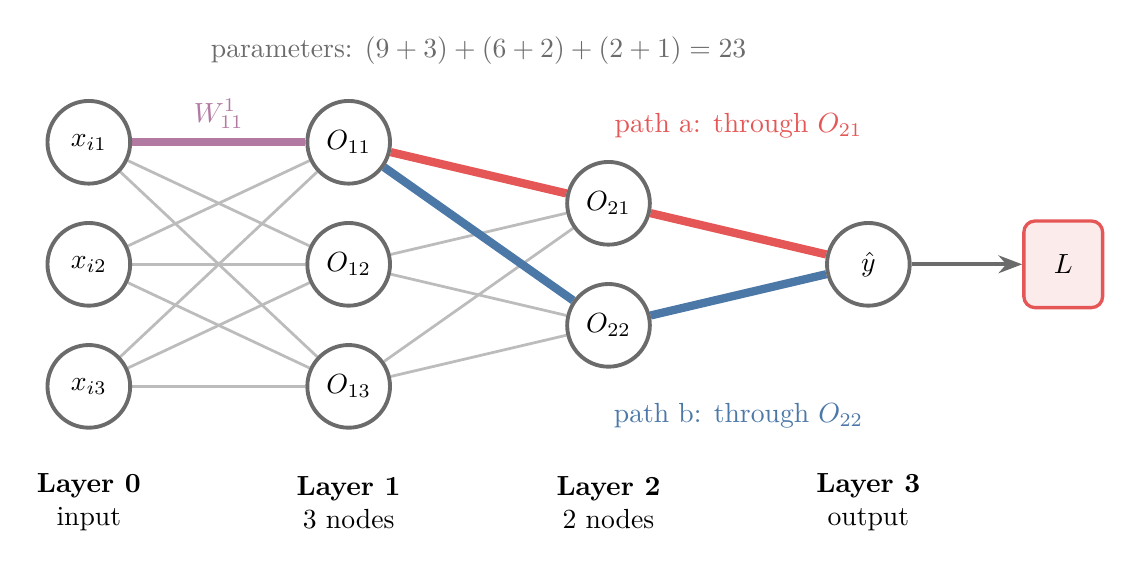
\begin{tikzpicture}[x=3.3cm, y=1.55cm,
  nd/.style={circle, draw=cgrey, fill=white, minimum size=1.05cm, line width=1.4pt, font=\sffamily},
  pa/.style={cred, line width=3pt}, pb/.style={cblue, line width=3pt}, both/.style={cpurple, line width=3pt}]
  \foreach \i in {1,2,3} \node[nd] (a\i) at (0, 2-\i) {$x_{i\i}$};
  \foreach \i in {1,2,3} \node[nd] (b\i) at (1, 2-\i) {$O_{1\i}$};
  \foreach \i in {1,2} \node[nd] (c\i) at (2, 1.5-\i) {$O_{2\i}$};
  \node[nd] (d) at (3, 0) {$\hat y$};
  \node[box=cred, minimum width=1cm] (L) at (3.75, 0) {$L$};
  \begin{scope}[on background layer]
    \foreach \i in {1,2,3} \foreach \j in {1,2,3} \draw[cgrey!45, line width=1pt] (a\i) -- (b\j);
    \foreach \i in {1,2,3} \foreach \j in {1,2} \draw[cgrey!45, line width=1pt] (b\i) -- (c\j);
    \foreach \i in {1,2} \draw[cgrey!45, line width=1pt] (c\i) -- (d);
    \draw[both] (a1) -- node[above, sloped, font=\sffamily, text=cpurple] {$W^{1}_{11}$} (b1);
    \draw[pa] (b1) -- (c1) -- (d);
    \draw[pb] (b1) -- (c2) -- (d);
  \end{scope}
  \draw[arrow] (d) -- (L);
  \node[font=\sffamily, text=cred, anchor=south] at (2.5, 0.95) {path a: through $O_{21}$};
  \node[font=\sffamily, text=cblue, anchor=north] at (2.5, -1.05) {path b: through $O_{22}$};
  \foreach \x/\t/\s in {0/Layer 0/input, 1/Layer 1/3 nodes, 2/Layer 2/2 nodes, 3/Layer 3/output}
    \node[align=center, font=\sffamily] at (\x, -1.95) {\textbf{\t}\\\s};
  \node[note, font=\sffamily\normalsize] at (1.5, 1.75) {parameters: $(9 + 3) + (6 + 2) + (2 + 1) = 23$};
\end{tikzpicture}
\end{document}
